\documentclass[12pt]{article}

\usepackage[english]{babel}
\usepackage{blindtext}
\usepackage{graphicx}
\usepackage{amssymb}
\usepackage{amsthm}
\usepackage{amsmath}
\usepackage{bbold}
%\textsc{•}\usepackage{bm}
%\usepackage{physics}
\usepackage[a4paper, width = 185mm, top = 15mm, bottom = 15mm]{geometry}
\usepackage{calligra}
\usepackage{float}
\usepackage{subcaption}
\usepackage{listings} 
\usepackage{xcolor}

\DeclareMathAlphabet{\mathcalligra}{T1}{calliga}{m}{n}
\DeclareFontShape{T1}{calligra}{m}{n}{<->s*[2.2]callig15}{}

\newcommand{\scripty}[1]{\ensuremath{\mathcalligra{#1}}}
\renewcommand* \d{\mathop{}\!\mathrm{d}}

\lstdefinestyle{mystyle}{
    language=Python,
    basicstyle=\ttfamily,
    keywordstyle=\color{blue},
    commentstyle=\color{green!60!black},
    stringstyle=\color{orange},
    showstringspaces=false,
    breaklines=true,
    frame=tb,
    backgroundcolor=\color{gray!10},
    numbers=left,
    numberstyle=\tiny\color{gray},
    tabsize=2,
    gobble=4,
}





\begin{document}
\noindent
\subsection*{Fixing of the Occupation and Chemical Potential}
\subsubsection*{Exact Diagonalization}
When solving the Hubbard dimer or just a chain of orbitals with nearest neighbour hopping along with a (non)local Coulomb interaction, using Exact Diagonalization in TRIQS, we take the following steps:
\begin{enumerate}
	\item Construct hopping maxtrix $t_{ij}$ and Coulomb tensor $V_{ijkl}$
	\item Construct the Hamiltonian $\hat{H}$ from $t_{ij}$ and $V_{ijkl}$ using creation- and annihilation-operators.
	\item Compute the atomic diagonal using \texttt{AtomDiagComplex}
	\item Compute the interacting Green's function using \texttt{atomic\_g\_iw}
\end{enumerate}
The obtained Green's function \texttt{G\_iw} has some occupation which we can compute using the \texttt{.total\_density()} method and taking only the real part. If there is no Coulomb interaction, which means $\hat{H}$ only consists of hopping terms, the resulting Green's function has the same occupation as the number of orbitals which is half-filling. This means that if we wish to have our system at an occupation that differs from half-filling, we'll have to change the chemical potential. Definitely so when we turn up the Coulomb interactions.\\
\\
Looking back at our steps for Exact Diagonalization, we have two places where we can adjust the chemical potential. We can add a term $\mu \hat{N}$ to the Hamiltonian at step 2, where $\hat{N}$ is the particle number operator. Or we can shift the chemical potential after step 4 by inverting the Green's function, adding the chemical potential and inverting again.
\subsubsection*{Chemical potential finder}
To know which chemical potential to choose, we can make a chemical potential finder which finds a chemical potential $\mu$ such that the occupation of the Green's function falls within a set tolerance \texttt{N\_tol} of the given \texttt{N\_fix} to which we want to fix the Green's function's occupation.
\begin{lstlisting}[style=mystyle]
    def chemical_potential_finder(g_w, N_fix, mu = 0, N_tol = 1e-6, ...):
    		g = chemical_potential_shift(g_w, mu, ...) # shifts g_w by mu
        occupation = N(g) # returns the occupation of g
        
        previous_direction = None
        step = abs(occupation - N_fix)
        
        while abs(occupation - N_fix) > N_tol:
            if occupation - N_fix > 0.0:
                if previous_direction == 'decrement':
                    step /= 2.0
                previous_direction = 'increment'
                mu += step
            if occupation - N_fix < 0.0:
                if previous_direction == 'increment':
                    step /= 2.0
                previous_direction = 'decrement'
                mu -= step
            
    				g = chemical_potential_shift(g_w, mu, ...)
        		occupation = N(g)
  
        return chemical_potential_shift(g_w, mu, ...)
\end{lstlisting}
\newpage
\noindent
So what we're doing is shifting the Green's function by a given $\mu$ which can just be set to zero and shifting here means adjusting the chemical potential, how this is done exactly doesn't matter for this algorithm, it's only designed to find the \textit{right} chemical potential. From this shifted Green's function we find its occupation and if it's not within the tolerance, we start changing the chemical potential, starting with a step that is the absolute value of the starting difference between the occupation and the desired occupation. We can also just set the step size to 1 for example, but a large discrepancy requires a larger step size and the other way around, so the absolute difference gives a reasonable step size.\\
It will first find the chemical potential by adding or subtracting this absolute difference, only when it overshoots in either direction, does the step size get cut in half. This way the chemical potential finder converges on a chemical potential in not too many steps.\\
\\
Going back to Exact Diagonalization, we can apply this chemical potential finder to either step 2 using an added term to the Hamilonian containing the chemical potential, or we can apply this finder to the final Green's function, or at both steps of course as in the first step the chemcical potential finding would happen at the \texttt{AtomDiagComplex} step, not at \texttt{atomic\_g\_iw}. Two solvers, one with fixing at step 2 and another with fixing at step 4, don't agree with eachother. A solver with both agrees with a solver that only fixes at step 2, so with a fixed \texttt{AtomDiagComplex}, the resulting Green's function from \texttt{atomic\_g\_iw} will have the same occupation still. (Not exactly equal)\\
I believe it makes the most physical sense to fix the chemical potential by adding the right term to the Hamiltonian and this would also mean the number of particles is 'fixed' before we actually perform the diagonalization. Therefore I'll use an Exact Diagonalization solver from now on where I've fixed the chemical potential at step 2.
\subsubsection*{Uniqueness and Analytical Continuation}
So we have a way of finding the chemical potential such that the occupation matches our desired occupation within a given tolerace. But if we look at the graph shown below, we see that the chemical potential is not unique for higher $\beta$ when it comes to finding the right occupation:
\begin{figure}[h!]
  \centering
  \begin{subfigure}[b]{0.45\textwidth}
    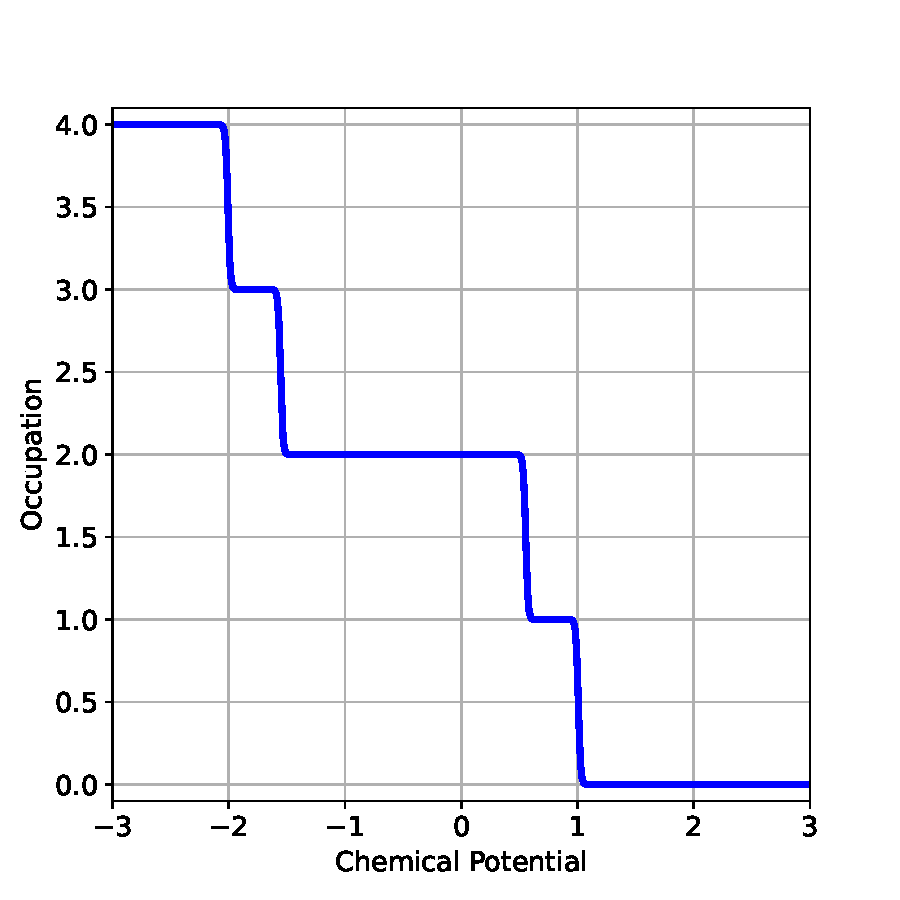
\includegraphics[width=\textwidth]{o2100.pdf}
    \caption{2 orbitals, $t=U=1.0$, $\beta = 100$}
  \end{subfigure}
  \hspace{0.02\textwidth}
  \begin{subfigure}[b]{0.45\textwidth}
    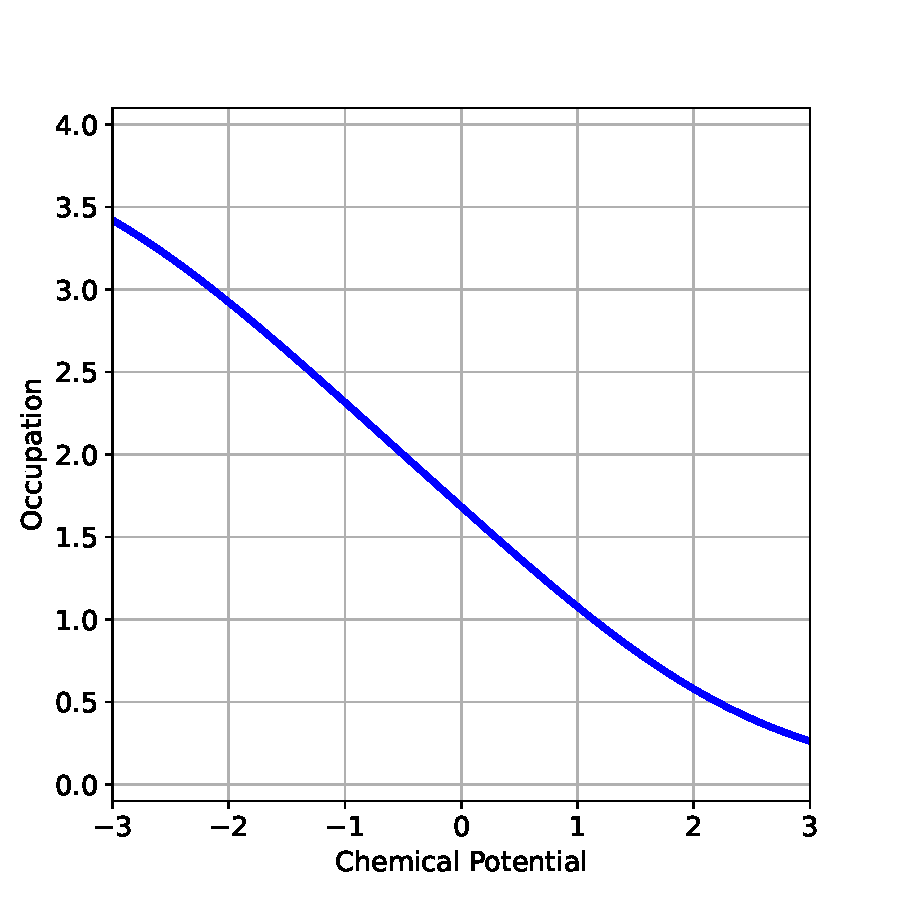
\includegraphics[width=\textwidth]{o21.pdf}
    \caption{2 orbitals, $t=U=1.0$, $\beta = 1$}
  \end{subfigure}
\end{figure}\\
So at higher $\beta$, there is a plateau of values for the chemical potential for which the Green's function has the same occupation, for lower $\beta\sim 1$, these plateaus dissapear. Physically there shouldn't be a difference between solutions with the same occupation even though if one would compare the Matusbara Green's functions directly, they do not agree because there is a shift inside the denominator by the chemical potential.
\newpage
\noindent
If we instead look at the Green's functions in real-frequency after using Pade to do the analytical continuation back to real frequncy, we can see the only difference is a shift because if we overlap them, they agree again:
\begin{figure}[h!]
\centering
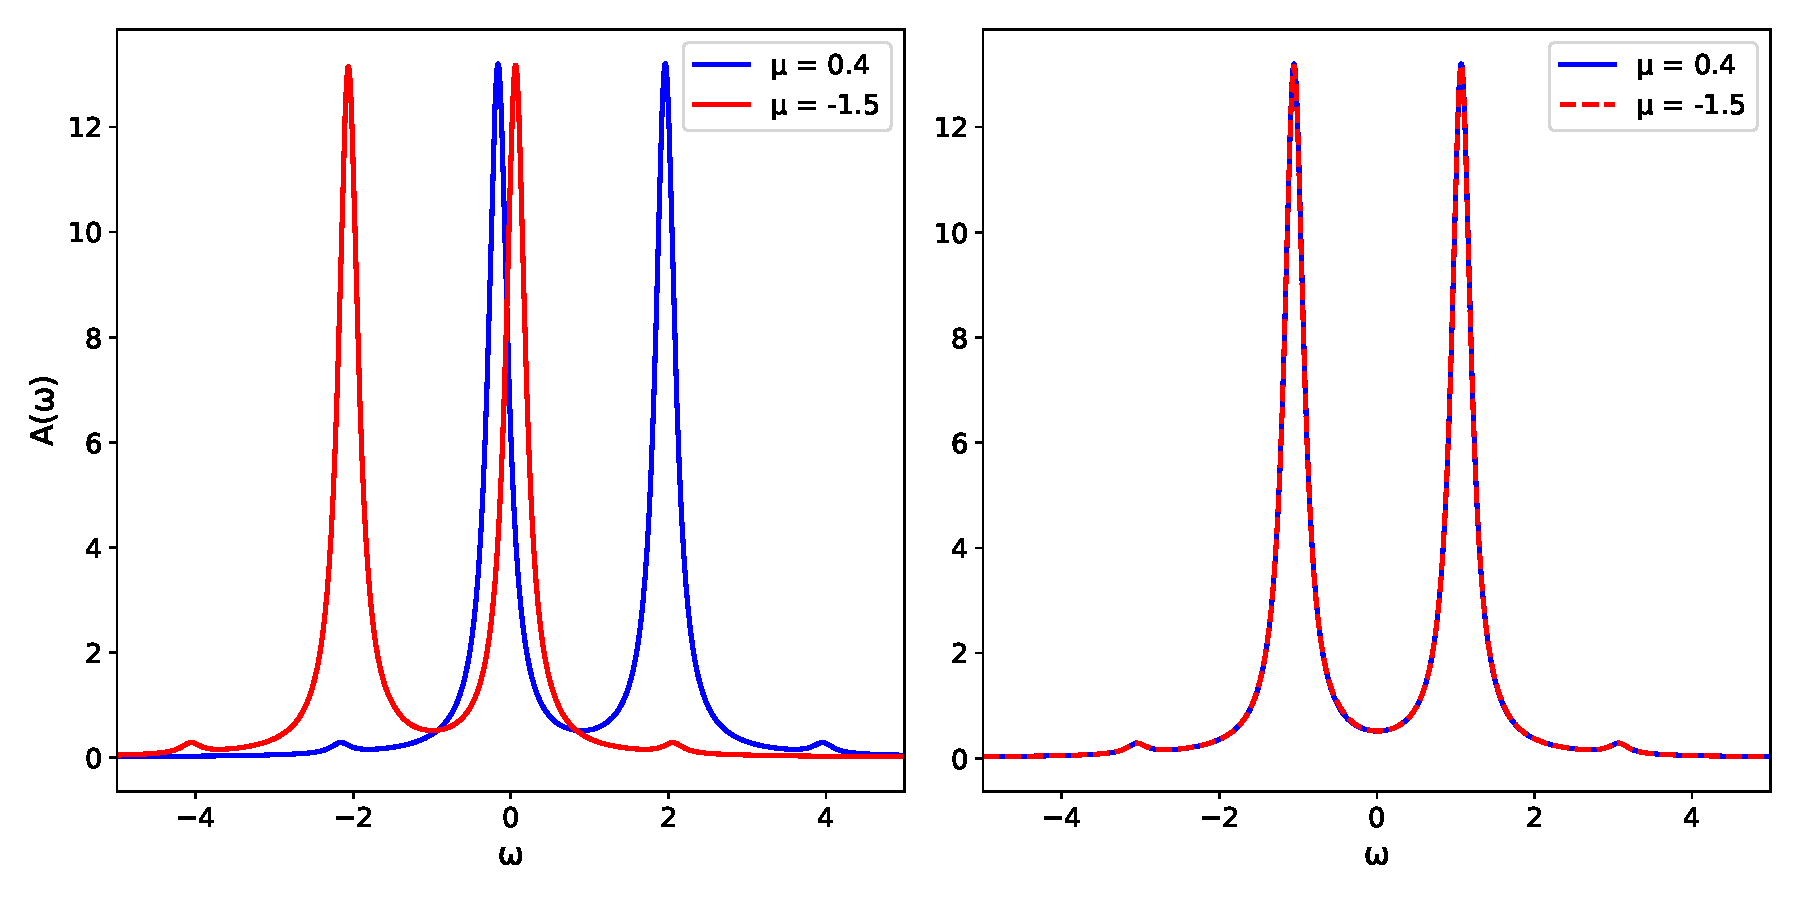
\includegraphics[width=\textwidth]{spec.pdf}
\caption{Left: Spectral function plots after Pade. Right: Same plots but both centered around $\omega=0$.}
\end{figure}\\
So we can see that even though we use a different chemical potential which causes the two Matsubara Green's functions to look totally different, the spectral functions of the analytically continuated imaginary frequency Green's functions only differ by an overal shift while the distance between the peaks remains the same. This means we can say that both Matsubara Green's functions are 'correct' as they give the same physics. Though this only really happens at high $\beta$ because of the plateau of possible values for the chemical potential which keep the occupation the same. As soon as the occupation differs between the two Green's functions, they no longer agree within a shift.\\
\\
In conclusion; for Exact Diagonalization we fix the chemical potential by adding a term to the Hamlitionian before doing the diagonalization. For higher $\beta$ we have a plateau of possible chemical potentials which in the end only differ by a shift in the spetral function, as long as the occupation is the same.
\subsubsection*{GW}
When doing GW calculations, we have a different set of steps:
\begin{enumerate}
	\item Start construcing $G_{ij}^0(i\omega)=[i\omega -t_{ij}]^{-1}$
	\item Calculate $P$, $W$, $\Sigma_\text{dyn}$, $\Sigma_\text{H}$ and $\Sigma_\text{F}$ from $G^0$
	\item Calculate the interacting $G$ by inverting the Dyson equation
	\item Optional: Iterate using the found $G$ until convergence
\end{enumerate}
When fixing the chemical potential for GW we have a few places where we can do so. We can fix the chemical potential of $G^0$ after step 1. $G^0$ will automatically be at half-filling so if we wish to deviate from half-filling, we'd have to fix the chemical potential. We can also fix the chemical potential of the computed interacting Green's function $G$ and this is necessary as after a one-shot GW, the occupation changes from that of $G^0$.
\newpage
\noindent
If we start to iterate we could fix the chemical potential at each iteration or only at the final iteration. But since we treat the found interacting $G$ as the new $G^0$ for the next iteration, it makes sense to fix the chemical potential at each iteration which automatically means it's fixed at the end.\\
\\
So fixing the chemical potential of $G^0$ and then $G$ at every iteration (including one-shot) seems the most correct physics wise and it gives decent agreement with Exact diagonalization. We again have that the solutions in Matusbara frequency look totally different, but once analytically continuated back to real frequency, the solutions agree bar a shift. (as much as one can expect GW to agree to the exact solution).

Below are some plots to show the results of the solver:
\begin{figure}[h!]
  \centering
  \begin{subfigure}[b]{0.45\textwidth}
    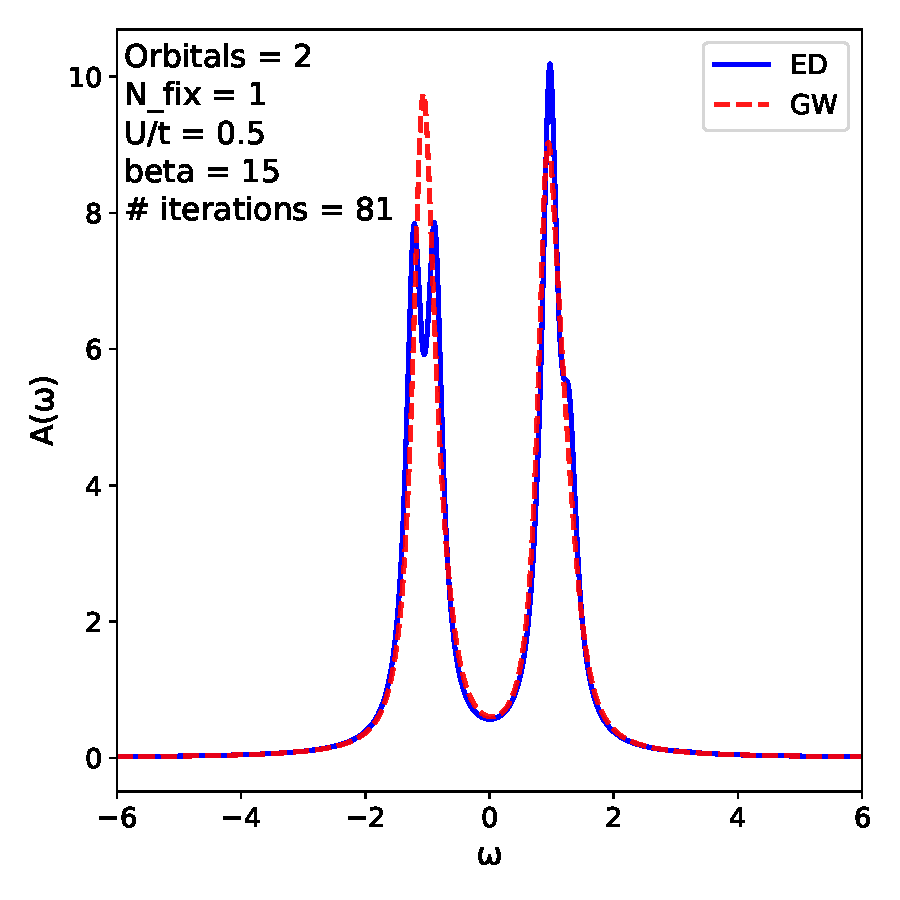
\includegraphics[width=\textwidth]{specgw21.pdf}
  \end{subfigure}
  \hspace{0.02\textwidth}
  \begin{subfigure}[b]{0.45\textwidth}
    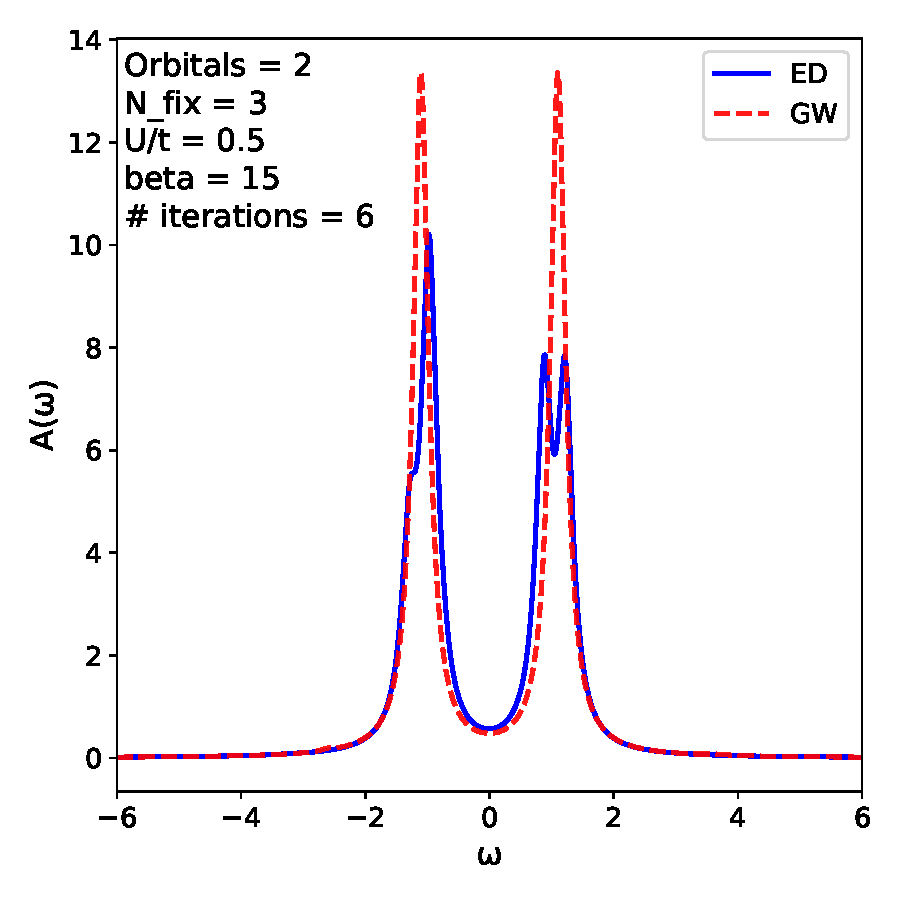
\includegraphics[width=\textwidth]{specgw23.pdf}
  \end{subfigure}
  \hspace{0.05\textwidth}
    \begin{subfigure}[b]{0.45\textwidth}
    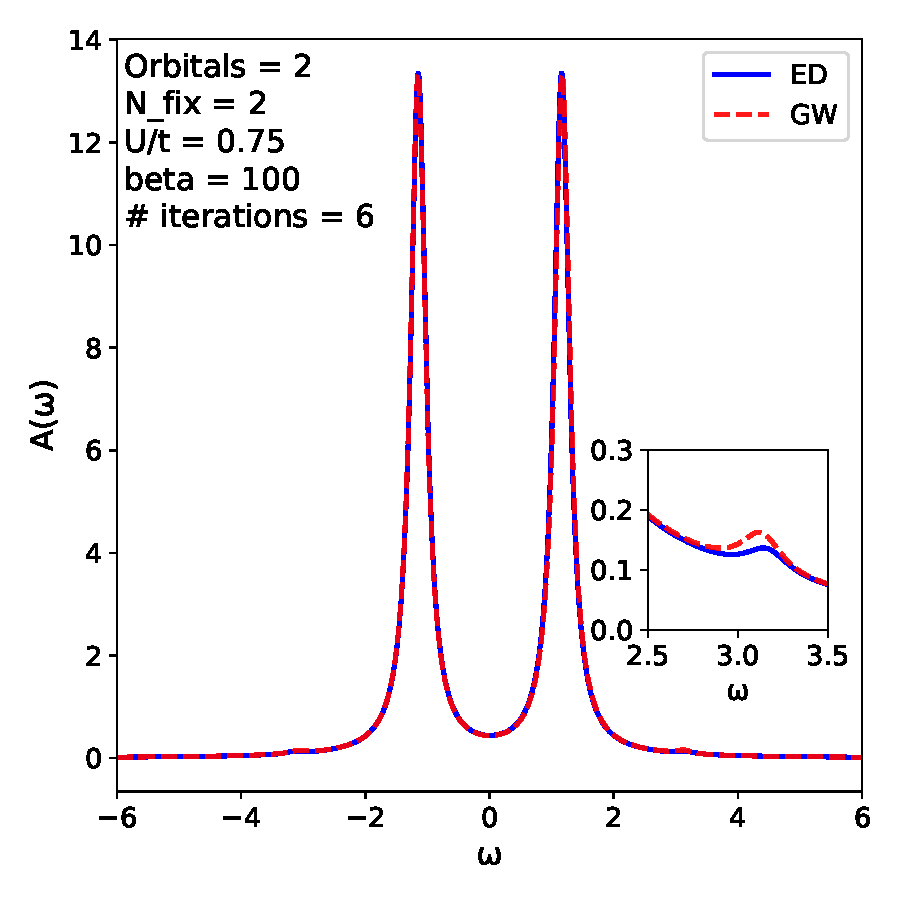
\includegraphics[width=\textwidth]{specgw22.pdf}
  \end{subfigure}
  \hspace{0.02\textwidth}
  \begin{subfigure}[b]{0.45\textwidth}
    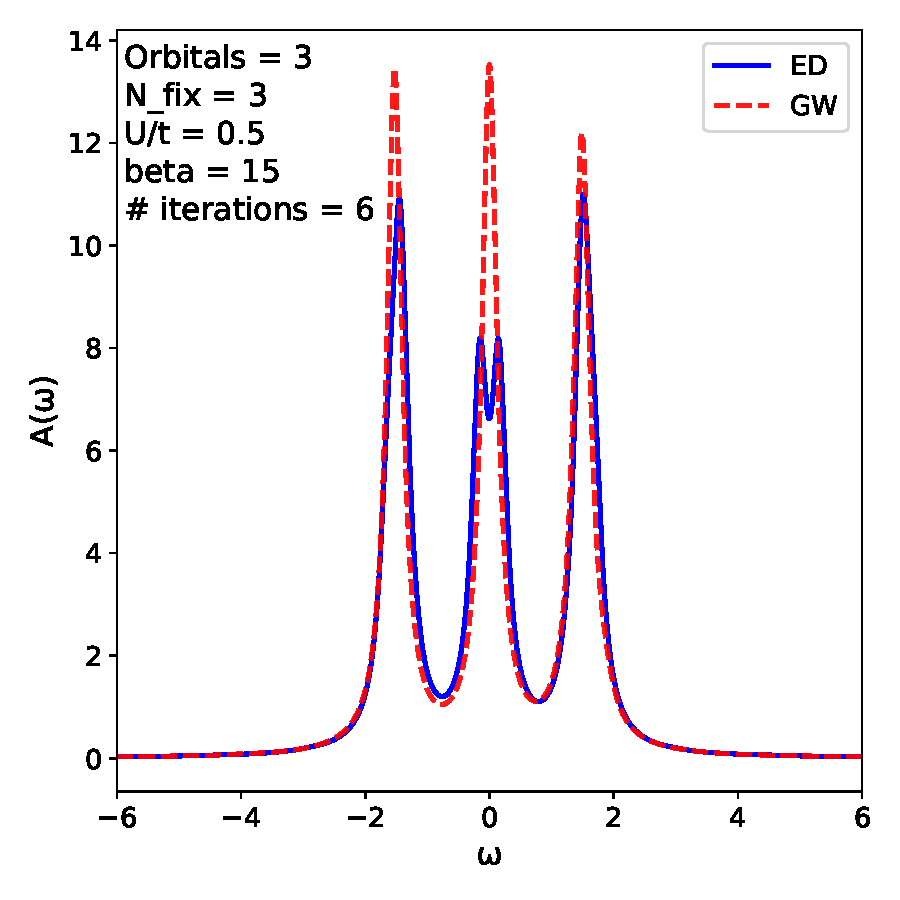
\includegraphics[width=\textwidth]{specgw33.pdf}
  \end{subfigure}
\end{figure}\\

\begin{figure}[h!]
  \centering
  \begin{subfigure}[b]{0.45\textwidth}
    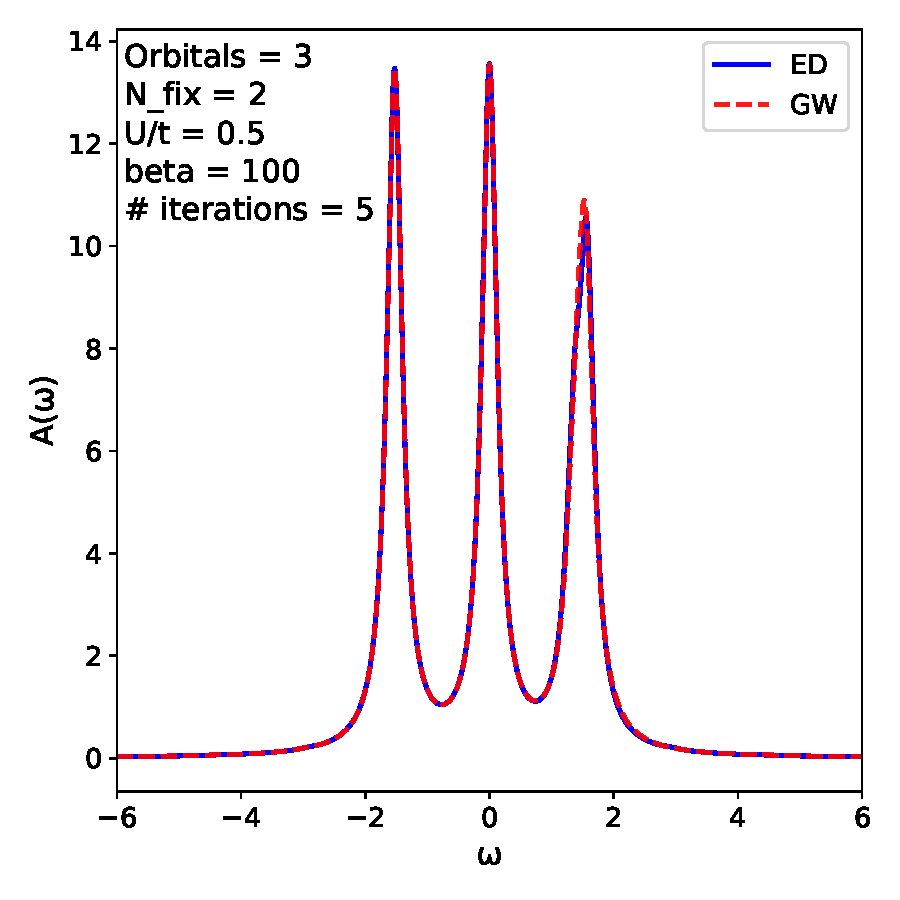
\includegraphics[width=\textwidth]{specgw32.pdf}
  \end{subfigure}
  \hspace{0.02\textwidth}
  \begin{subfigure}[b]{0.45\textwidth}
    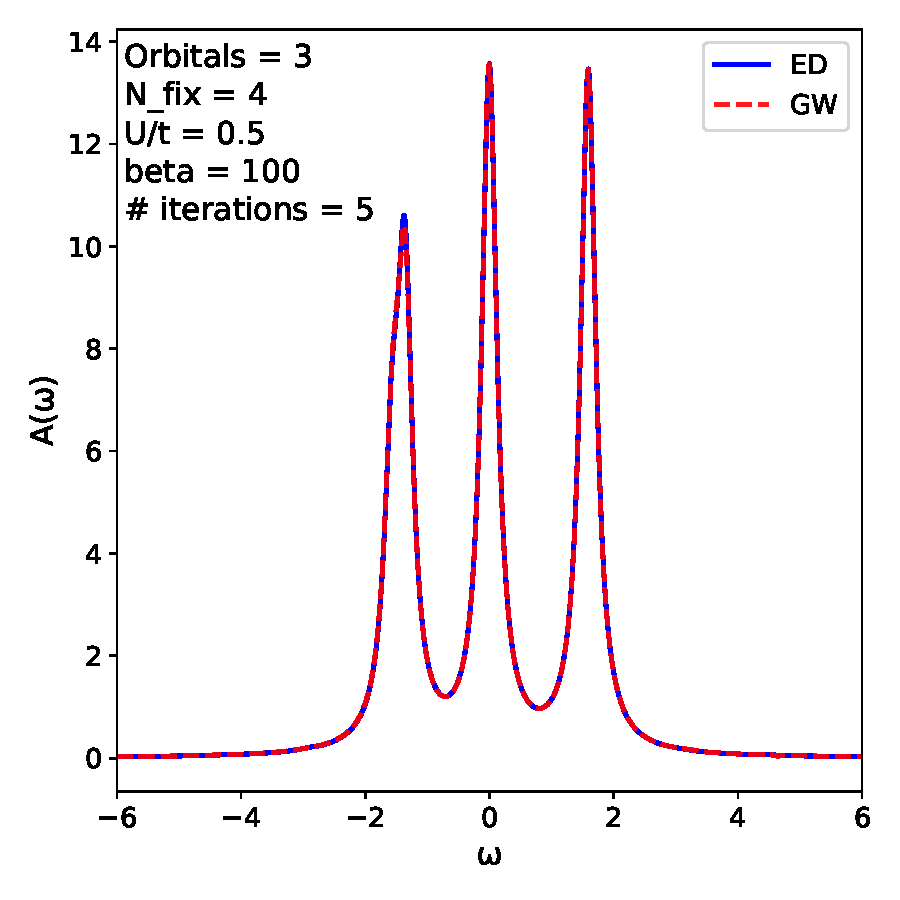
\includegraphics[width=\textwidth]{specgw34.pdf}
  \end{subfigure}
  \hspace{0.05\textwidth}
    \begin{subfigure}[b]{0.45\textwidth}
    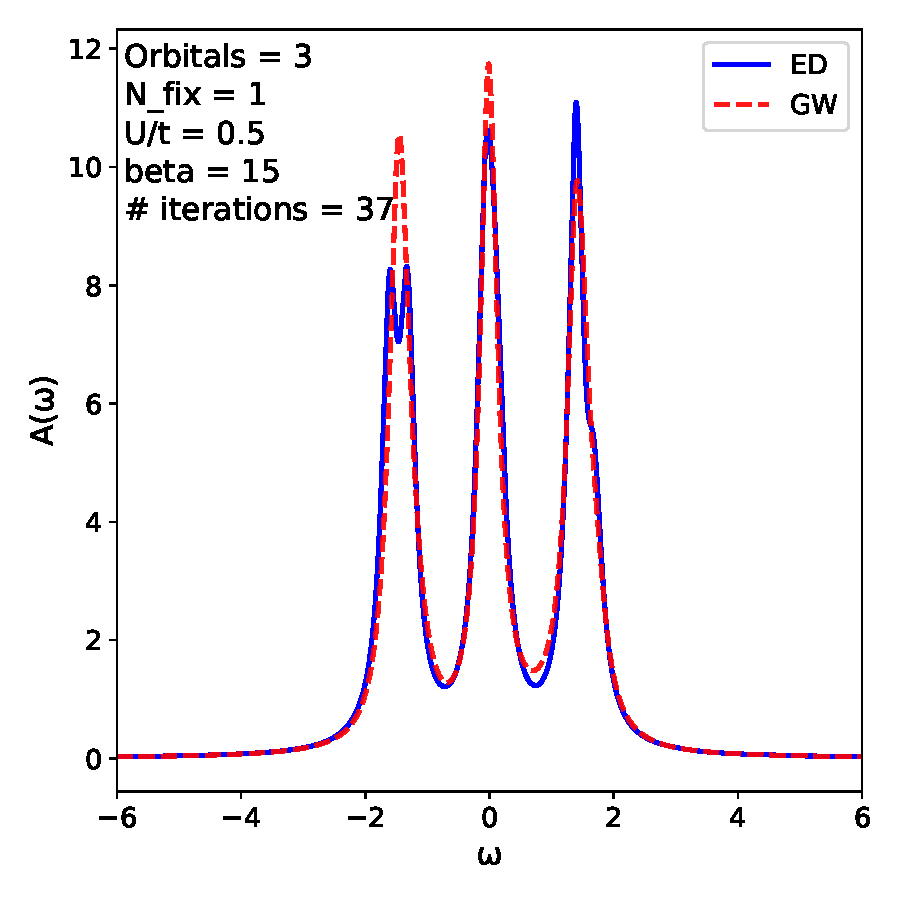
\includegraphics[width=\textwidth]{specgw31.pdf}
  \end{subfigure}
  \hspace{0.02\textwidth}
  \begin{subfigure}[b]{0.45\textwidth}
    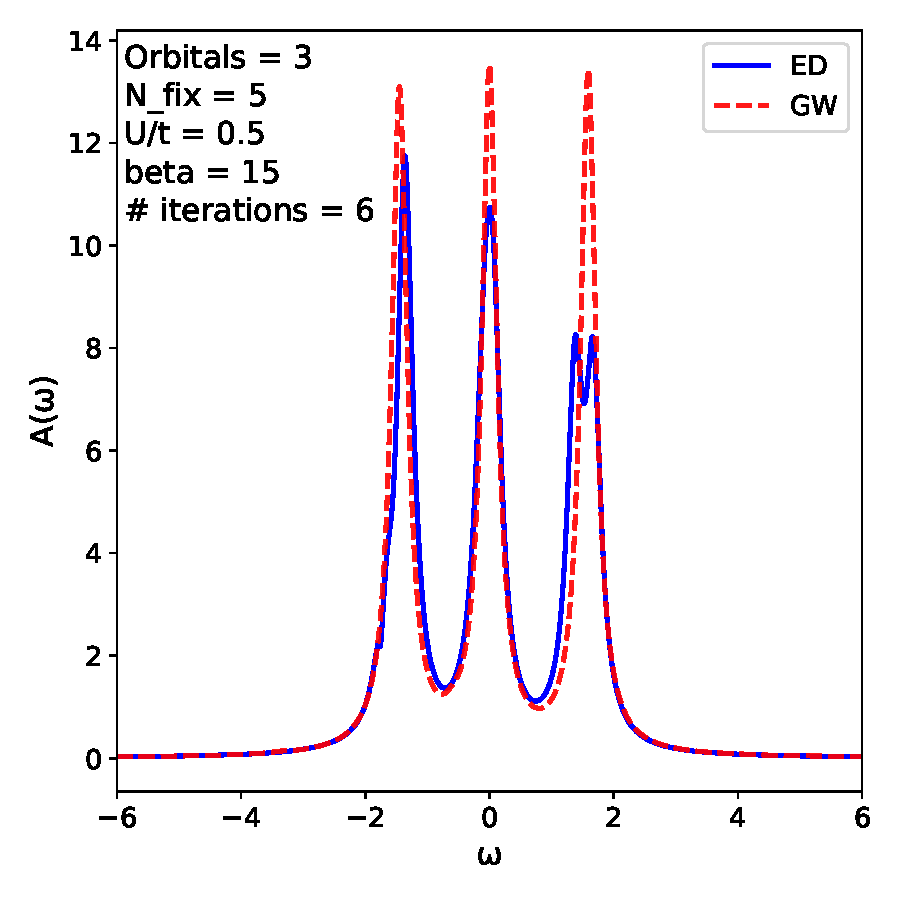
\includegraphics[width=\textwidth]{specgw35.pdf}
  \end{subfigure}
\end{figure}
\end{document}
